\documentclass[12pt,prb,aps,epsf]{article}
\usepackage[utf8]{inputenc}
\usepackage{amsmath}
\usepackage{amsfonts}
\usepackage{amssymb}
\usepackage{graphicx} 
\usepackage{latexsym} 
\usepackage[toc,page]{appendix}
\usepackage{listings}
\usepackage{xcolor}
\usepackage{soul}
\usepackage[T1]{fontenc}
\usepackage{amsthm}
\usepackage{mathtools}
\usepackage{setspace}
\usepackage{array,multirow,makecell}
\usepackage{geometry}
\usepackage{textcomp}
\usepackage{float}
%\usepackage{siunitx}
\usepackage{cancel}
%\usepackage{tikz}
%\usetikzlibrary{calc, shapes, backgrounds, arrows, decorations.pathmorphing, positioning, fit, petri, tikzmark}
\usepackage{here}
\usepackage{titlesec}
%\usepackage{bm}
\usepackage{bbold}

\geometry{hmargin=2cm,vmargin=2cm}

\begin{document}
	
	\title{MP 28 Instabilités et phénomènes non linéaires}
	\author{Naïmo Davier}
	
	\maketitle
	
	\tableofcontents
	
	\pagebreak
	
\subsection{Introduction}	
Les équations linéaires ne sont généralement qu'une approximation, souvent pour un domaine de paramètres donnés, des équation non linéaires qui régissent le monde (en supposant qu'il soit bel et bien possible de représenter le monde avec des équations mais on tend là vers la philo). On va montrer dans ce montage différents exemples expérimentalement simples à mettre en place mais permettant de mettre en valeur différents aspects de la physique non linéaire.


\section{Pendule pesant}
Voir BUP 867.\\

On étudie dans cette section le cas d'un pendule pesant constitué d'une tige rigide avec une masse au bout de celle ci, et dont l'axe est relié à un potentiomètre qui nous permet donc d'analyser avec latispro une tension $U(\theta)$ nous permettant de remonter à $\theta(t)$ en étalonnant le potentiomètre pour quelques angles donnés (en général -90°, 0° et 90°).\\

Le branchement du potentiomètre est en général pris en $-15V, +U$ avec U de l'ordre de $10-15V$, en effet la sensibilité dépend de la différence de tension, que l'on souhaite donc maximale. $U_s$ pouvant alors varier environ de $25V$ entre $-\pi$ et $\pi$ on pourra réduire cet écart de tension si on veut analyser des mouvements de très grande amplitude pour que la carte d'acquisition ne sature pas ($-10V,+10V$), mais cette gamme de tension convient parfaitement pour des amplitudes max de l'ordre de $\pi/2$. On règlera ensuite $U$ de telle sorte à ce que la valeur moyenne de U soit nulle, avant d'étalonner le potentiomètre pour avoir $\theta(U_s)$ sur latispro.

\begin{figure}[h]
	\centerline{\includegraphics[width=8cm]{pendule}}
\end{figure}
\subsection{Perte de l'isochronisme}
On relève la période $T$ des oscillations en fonction de l'amplitude $\theta_{max}$ pour tracer $T(\theta_{max}$ sur régressi, à comparer avec la formule de Borda 
\begin{eqnarray}
T = T_0\left(1 + \frac{\theta_{max}^2}{16}\right)
\end{eqnarray}
On montre alors la perte d'isochronisme dès que les angles dépasse une vingtaine de degrés : la linéarisation des équations n'est plus possible.\\

Pour obtenir la formule de Borda on peu se référer au calcul de la leçon n°49 ou bien préférer passer par la conservation de l'énergie 
\begin{eqnarray}
E = \frac{1}{2} I\dot{\theta}^2 + mgl (1-\cos(\theta)) = mgl(1-\cos(\theta_{0}))
\end{eqnarray}
avec $\theta_0$ l'amplitude des oscillations. On a alors 
\begin{eqnarray}
\dot{\theta} = \frac{d\theta}{dt} = \sqrt{\frac{2mgl}{I}[\cos(\theta) - \cos(\theta_0)]}\;\;\Longrightarrow \;\; dt = \frac{d\theta}{\sqrt{\frac{2mgl}{I}[\cos(\theta) - \cos(\theta_0)]}}\\
\Rightarrow \frac{T}{4} = \int_{0}^{\theta_0} \frac{d\theta}{\sqrt{\frac{2mgl}{I}[\cos(\theta) - \cos(\theta_0)]}} 
\end{eqnarray}
Cette expression de la période est exacte, et on peut en faire une développement à l'aide d'un logiciel de calcul formel pur établir la formule de Borda.

\subsection{Perte d'harmonicité}
On peut montrer la perte d'harmonicité en enregistrant une petite dizaine d'oscillation d'une grande amplitude (au moins 70° si on veut espérer le voir), et en regardant la TF de $\dot{\theta}$, en effet on s'attend à avoir (v LP 49)
\begin{eqnarray}
\theta(t) \simeq \theta_{max}\sin(\omega t) + \frac{\theta_{max}^2}{192}\sin(3\omega t)\\
\rightarrow \dot{\theta}(t) \simeq \omega\left(\theta_m\cos(\omega t) + 3\frac{\theta_m^2}{192}\cos(3\omega t) \right)
\end{eqnarray}
on est donc sensé observé un pic à $3\omega$ 3 fois plus intense sur la TF de $\dot{\theta}$ que sur celle de $\theta$.\\
La mesure consistera à mesurer l'amplitude relative du pic à $3\omega$ par rapport au fondamental et à la comparer à celle attendue donnée ci dessus.

\section{Oscillateur paramétrique}
Voir BUP 747 (version PDF dans le dossier), il y a les explications et indications nécessaires.

\section{Oscillateur à boules - Pendule conique}

La physique est similaire dans les deux cas :\\
On a un pendule simple accroché en haut dans axe tournant à la vitesse angulaire $\omega$.\\

 Lorsque $\omega < \omega_c$ la masse reste le long de l'axe : la gravité l'emporte sur la force centrifuge et il n'y a qu'un seul point stable en $\theta =0$ (où $\theta$ est l'angle que fait le pendule avec l'axe de rotation = verticale). \\
 
 Lorsque $\omega > \omega_c$ on a alors la masse qui décolle : il y a deux nouvelles positions d'équilibre stable $\theta = \pm\theta_e$ qui correspondent à l'équilibre entre gravité et force centrifuge : 
 \begin{eqnarray}
 \vec{P} = m\vec{g}\hspace{1cm}\mathrm{et}\hspace{1cm}\vec{F}_c = md\omega^2\vec{e}_{\perp}
 \end{eqnarray}
où $d = l\sin{\theta}$ est la distance du centre de gravité de la masse à l'axe, et $\vec{e}_{\perp}$ le vecteur orthogonal à la verticale attaché au pendule. On a alors à l'équilibre, selon $\vec{e}_{\theta}$ :
\begin{eqnarray}
mg\sin(\theta_e) = ml\sin(\theta_e)\omega^2\cos(\theta_e)\\
\cos\theta_e \simeq 1 - \frac{\theta^2}{2} = \frac{g/l}{\omega^2}\\
\Longrightarrow \theta_e \simeq \sqrt{2\left(1-\frac{g/l}{\omega^2}\right) }
\end{eqnarray} 

L'idée est donc de relever plusieurs points afin de tracer $\theta_e(\omega)$, et de modéliser la courbe obtenue par 
\begin{eqnarray}
\theta_e = \alpha\sqrt{1-\beta/\omega^2}
\end{eqnarray}
pour déterminer $\alpha$ (supposé égal à $\sqrt{2}$) et $\beta$ qui représente $\omega_0= g/l$.\\

Le graphe obtenu est alors celui d'une bifurcation fourche, les lignes pleines représentant les points stables et les pointillés les points d'équilibre instables.
\begin{figure}[h]
	\centerline{\includegraphics[width=15cm]{fourche}}
\end{figure}

\end{document}